% Options for packages loaded elsewhere
\PassOptionsToPackage{unicode}{hyperref}
\PassOptionsToPackage{hyphens}{url}
\PassOptionsToPackage{dvipsnames,svgnames,x11names}{xcolor}
%
\documentclass[
  letterpaper,
  DIV=11,
  numbers=noendperiod]{scrreprt}

\usepackage{amsmath,amssymb}
\usepackage{lmodern}
\usepackage{iftex}
\ifPDFTeX
  \usepackage[T1]{fontenc}
  \usepackage[utf8]{inputenc}
  \usepackage{textcomp} % provide euro and other symbols
\else % if luatex or xetex
  \usepackage{unicode-math}
  \defaultfontfeatures{Scale=MatchLowercase}
  \defaultfontfeatures[\rmfamily]{Ligatures=TeX,Scale=1}
\fi
% Use upquote if available, for straight quotes in verbatim environments
\IfFileExists{upquote.sty}{\usepackage{upquote}}{}
\IfFileExists{microtype.sty}{% use microtype if available
  \usepackage[]{microtype}
  \UseMicrotypeSet[protrusion]{basicmath} % disable protrusion for tt fonts
}{}
\makeatletter
\@ifundefined{KOMAClassName}{% if non-KOMA class
  \IfFileExists{parskip.sty}{%
    \usepackage{parskip}
  }{% else
    \setlength{\parindent}{0pt}
    \setlength{\parskip}{6pt plus 2pt minus 1pt}}
}{% if KOMA class
  \KOMAoptions{parskip=half}}
\makeatother
\usepackage{xcolor}
\setlength{\emergencystretch}{3em} % prevent overfull lines
\setcounter{secnumdepth}{5}
% Make \paragraph and \subparagraph free-standing
\ifx\paragraph\undefined\else
  \let\oldparagraph\paragraph
  \renewcommand{\paragraph}[1]{\oldparagraph{#1}\mbox{}}
\fi
\ifx\subparagraph\undefined\else
  \let\oldsubparagraph\subparagraph
  \renewcommand{\subparagraph}[1]{\oldsubparagraph{#1}\mbox{}}
\fi

\usepackage{color}
\usepackage{fancyvrb}
\newcommand{\VerbBar}{|}
\newcommand{\VERB}{\Verb[commandchars=\\\{\}]}
\DefineVerbatimEnvironment{Highlighting}{Verbatim}{commandchars=\\\{\}}
% Add ',fontsize=\small' for more characters per line
\usepackage{framed}
\definecolor{shadecolor}{RGB}{241,243,245}
\newenvironment{Shaded}{\begin{snugshade}}{\end{snugshade}}
\newcommand{\AlertTok}[1]{\textcolor[rgb]{0.68,0.00,0.00}{#1}}
\newcommand{\AnnotationTok}[1]{\textcolor[rgb]{0.37,0.37,0.37}{#1}}
\newcommand{\AttributeTok}[1]{\textcolor[rgb]{0.40,0.45,0.13}{#1}}
\newcommand{\BaseNTok}[1]{\textcolor[rgb]{0.68,0.00,0.00}{#1}}
\newcommand{\BuiltInTok}[1]{\textcolor[rgb]{0.00,0.23,0.31}{#1}}
\newcommand{\CharTok}[1]{\textcolor[rgb]{0.13,0.47,0.30}{#1}}
\newcommand{\CommentTok}[1]{\textcolor[rgb]{0.37,0.37,0.37}{#1}}
\newcommand{\CommentVarTok}[1]{\textcolor[rgb]{0.37,0.37,0.37}{\textit{#1}}}
\newcommand{\ConstantTok}[1]{\textcolor[rgb]{0.56,0.35,0.01}{#1}}
\newcommand{\ControlFlowTok}[1]{\textcolor[rgb]{0.00,0.23,0.31}{#1}}
\newcommand{\DataTypeTok}[1]{\textcolor[rgb]{0.68,0.00,0.00}{#1}}
\newcommand{\DecValTok}[1]{\textcolor[rgb]{0.68,0.00,0.00}{#1}}
\newcommand{\DocumentationTok}[1]{\textcolor[rgb]{0.37,0.37,0.37}{\textit{#1}}}
\newcommand{\ErrorTok}[1]{\textcolor[rgb]{0.68,0.00,0.00}{#1}}
\newcommand{\ExtensionTok}[1]{\textcolor[rgb]{0.00,0.23,0.31}{#1}}
\newcommand{\FloatTok}[1]{\textcolor[rgb]{0.68,0.00,0.00}{#1}}
\newcommand{\FunctionTok}[1]{\textcolor[rgb]{0.28,0.35,0.67}{#1}}
\newcommand{\ImportTok}[1]{\textcolor[rgb]{0.00,0.46,0.62}{#1}}
\newcommand{\InformationTok}[1]{\textcolor[rgb]{0.37,0.37,0.37}{#1}}
\newcommand{\KeywordTok}[1]{\textcolor[rgb]{0.00,0.23,0.31}{#1}}
\newcommand{\NormalTok}[1]{\textcolor[rgb]{0.00,0.23,0.31}{#1}}
\newcommand{\OperatorTok}[1]{\textcolor[rgb]{0.37,0.37,0.37}{#1}}
\newcommand{\OtherTok}[1]{\textcolor[rgb]{0.00,0.23,0.31}{#1}}
\newcommand{\PreprocessorTok}[1]{\textcolor[rgb]{0.68,0.00,0.00}{#1}}
\newcommand{\RegionMarkerTok}[1]{\textcolor[rgb]{0.00,0.23,0.31}{#1}}
\newcommand{\SpecialCharTok}[1]{\textcolor[rgb]{0.37,0.37,0.37}{#1}}
\newcommand{\SpecialStringTok}[1]{\textcolor[rgb]{0.13,0.47,0.30}{#1}}
\newcommand{\StringTok}[1]{\textcolor[rgb]{0.13,0.47,0.30}{#1}}
\newcommand{\VariableTok}[1]{\textcolor[rgb]{0.07,0.07,0.07}{#1}}
\newcommand{\VerbatimStringTok}[1]{\textcolor[rgb]{0.13,0.47,0.30}{#1}}
\newcommand{\WarningTok}[1]{\textcolor[rgb]{0.37,0.37,0.37}{\textit{#1}}}

\providecommand{\tightlist}{%
  \setlength{\itemsep}{0pt}\setlength{\parskip}{0pt}}\usepackage{longtable,booktabs,array}
\usepackage{calc} % for calculating minipage widths
% Correct order of tables after \paragraph or \subparagraph
\usepackage{etoolbox}
\makeatletter
\patchcmd\longtable{\par}{\if@noskipsec\mbox{}\fi\par}{}{}
\makeatother
% Allow footnotes in longtable head/foot
\IfFileExists{footnotehyper.sty}{\usepackage{footnotehyper}}{\usepackage{footnote}}
\makesavenoteenv{longtable}
\usepackage{graphicx}
\makeatletter
\def\maxwidth{\ifdim\Gin@nat@width>\linewidth\linewidth\else\Gin@nat@width\fi}
\def\maxheight{\ifdim\Gin@nat@height>\textheight\textheight\else\Gin@nat@height\fi}
\makeatother
% Scale images if necessary, so that they will not overflow the page
% margins by default, and it is still possible to overwrite the defaults
% using explicit options in \includegraphics[width, height, ...]{}
\setkeys{Gin}{width=\maxwidth,height=\maxheight,keepaspectratio}
% Set default figure placement to htbp
\makeatletter
\def\fps@figure{htbp}
\makeatother

\KOMAoption{captions}{tableheading}
\makeatletter
\makeatother
\makeatletter
\@ifpackageloaded{bookmark}{}{\usepackage{bookmark}}
\makeatother
\makeatletter
\@ifpackageloaded{caption}{}{\usepackage{caption}}
\AtBeginDocument{%
\ifdefined\contentsname
  \renewcommand*\contentsname{Table of contents}
\else
  \newcommand\contentsname{Table of contents}
\fi
\ifdefined\listfigurename
  \renewcommand*\listfigurename{List of Figures}
\else
  \newcommand\listfigurename{List of Figures}
\fi
\ifdefined\listtablename
  \renewcommand*\listtablename{List of Tables}
\else
  \newcommand\listtablename{List of Tables}
\fi
\ifdefined\figurename
  \renewcommand*\figurename{Figure}
\else
  \newcommand\figurename{Figure}
\fi
\ifdefined\tablename
  \renewcommand*\tablename{Table}
\else
  \newcommand\tablename{Table}
\fi
}
\@ifpackageloaded{float}{}{\usepackage{float}}
\floatstyle{ruled}
\@ifundefined{c@chapter}{\newfloat{codelisting}{h}{lop}}{\newfloat{codelisting}{h}{lop}[chapter]}
\floatname{codelisting}{Listing}
\newcommand*\listoflistings{\listof{codelisting}{List of Listings}}
\makeatother
\makeatletter
\@ifpackageloaded{caption}{}{\usepackage{caption}}
\@ifpackageloaded{subcaption}{}{\usepackage{subcaption}}
\makeatother
\makeatletter
\@ifpackageloaded{tcolorbox}{}{\usepackage[many]{tcolorbox}}
\makeatother
\makeatletter
\@ifundefined{shadecolor}{\definecolor{shadecolor}{rgb}{.97, .97, .97}}
\makeatother
\makeatletter
\makeatother
\ifLuaTeX
  \usepackage{selnolig}  % disable illegal ligatures
\fi
\IfFileExists{bookmark.sty}{\usepackage{bookmark}}{\usepackage{hyperref}}
\IfFileExists{xurl.sty}{\usepackage{xurl}}{} % add URL line breaks if available
\urlstyle{same} % disable monospaced font for URLs
\hypersetup{
  pdftitle={Berk Özcan Progress Journal},
  colorlinks=true,
  linkcolor={blue},
  filecolor={Maroon},
  citecolor={Blue},
  urlcolor={Blue},
  pdfcreator={LaTeX via pandoc}}

\title{Berk Özcan Progress Journal}
\author{}
\date{}

\begin{document}
\maketitle
\ifdefined\Shaded\renewenvironment{Shaded}{\begin{tcolorbox}[borderline west={3pt}{0pt}{shadecolor}, enhanced, boxrule=0pt, breakable, sharp corners, frame hidden, interior hidden]}{\end{tcolorbox}}\fi

\renewcommand*\contentsname{Table of contents}
{
\hypersetup{linkcolor=}
\setcounter{tocdepth}{2}
\tableofcontents
}
\bookmarksetup{startatroot}

\hypertarget{introduction}{%
\chapter*{Introduction}\label{introduction}}
\addcontentsline{toc}{chapter}{Introduction}

\markboth{Introduction}{Introduction}

This progress journal covers BERK ÖZCAN's work during their term at
\href{https://mef-bda503.github.io/fall22/}{BDA 503 Fall 2022}.

Each section is an assignment or an individual work.

\bookmarksetup{startatroot}

\hypertarget{assignment-1}{%
\chapter{Assignment 1}\label{assignment-1}}

Berk Özcan, I've been working as a Senior Data Analyst in Doğuş
Teknoloji for almost 2 years. I have 5 years of experience in Analytical
departments, before that, I worked as a merchandise planner in several
retail companies. One of my biggest aim is after this program, I want to
get a promotion to become Analytics Manager. I work with mostly SQL and
Python in my current job. With my new skills I believe that I can handle
complex problems, also in this field we always have to get to update our
knowledge and I could enhance my understanding of data and analytics
through my education.

\href{https://www.linkedin.com/in/berk-\%C3\%B6zcan-b6b19a13b}{\textbf{My
linkedin profile}}

\hypertarget{user-2022---tutorials--introduction-to-git-and-github-tutorial-}{%
\section{useR! 2022 - Tutorials -Introduction to Git and GitHub
Tutorial-}\label{user-2022---tutorials--introduction-to-git-and-github-tutorial-}}

\href{https://www.youtube.com/watch?v=U186T7U08sA\&list=PL77T87Q0eoJhQDXzG2Viq3uHf5YyJfw0L\&index=5}{\emph{Here
is the link}}

I preferred to watch an introduction video about Git and GitHub. In this
video, we can learn the usage of Git and GitHub, why they are important
in our life and some bash codes for administrating the pipeline.

Firstly we should understand the notion of version control. With version
control, we can manage changes to projects over time, and also we can
track changes to files.

There are several reasons why we are using version control:

\begin{enumerate}
\def\labelenumi{\arabic{enumi})}
\tightlist
\item
  Collaboration : Simultaneously work on the same orıject
\item
  Tracking : Record the development of a project
\item
  Restoring versions : Restore older versions of a file
\item
  Back-up : Save your work in a remote repository.
\end{enumerate}

WHY GIT:

-Second generation version control system -Unique approach to tracking
changes -Streamlined collaboration -Manages evolution of a project -Fast
and lightweight branching -Commit messages provide context -Safe testing
and experimentation

WHY GITHUB

-Provides cloud storage for our project -Like dropbox but with better
features -It allows us to: \emph{view and review our work} sync with a
project *report issues/bugs -contribute to the project -Great way to
promote our skills and interests

Some Git Terms we have to know

\emph{Repository} Commit \emph{Push/Pull} Branch \emph{Pull/Merge
request} Issues

With this suggested video also ensures how can we use the tool with
bash/shell codes.

\hypertarget{r-posts-relevant-to-my-interests}{%
\section{R posts relevant to my
interests}\label{r-posts-relevant-to-my-interests}}

\hypertarget{basic-visualization-with-r}{%
\subsection{Basic Visualization with
R}\label{basic-visualization-with-r}}

\begin{Shaded}
\begin{Highlighting}[]
\DocumentationTok{\#\#\# Histogram}

\FunctionTok{data}\NormalTok{(airquality)}
  
\FunctionTok{hist}\NormalTok{(airquality}\SpecialCharTok{$}\NormalTok{Temp, }\AttributeTok{main =}\StringTok{"La Guardia Airport\textquotesingle{}s\textbackslash{}}
\StringTok{Maximum Temperature(Daily)"}\NormalTok{,}
    \AttributeTok{xlab =}\StringTok{"Temperature(Fahrenheit)"}\NormalTok{,}
    \AttributeTok{xlim =} \FunctionTok{c}\NormalTok{(}\DecValTok{50}\NormalTok{, }\DecValTok{125}\NormalTok{), }\AttributeTok{col =}\StringTok{"yellow"}\NormalTok{,}
    \AttributeTok{freq =} \ConstantTok{TRUE}\NormalTok{)}
\end{Highlighting}
\end{Shaded}

\begin{figure}[H]

{\centering 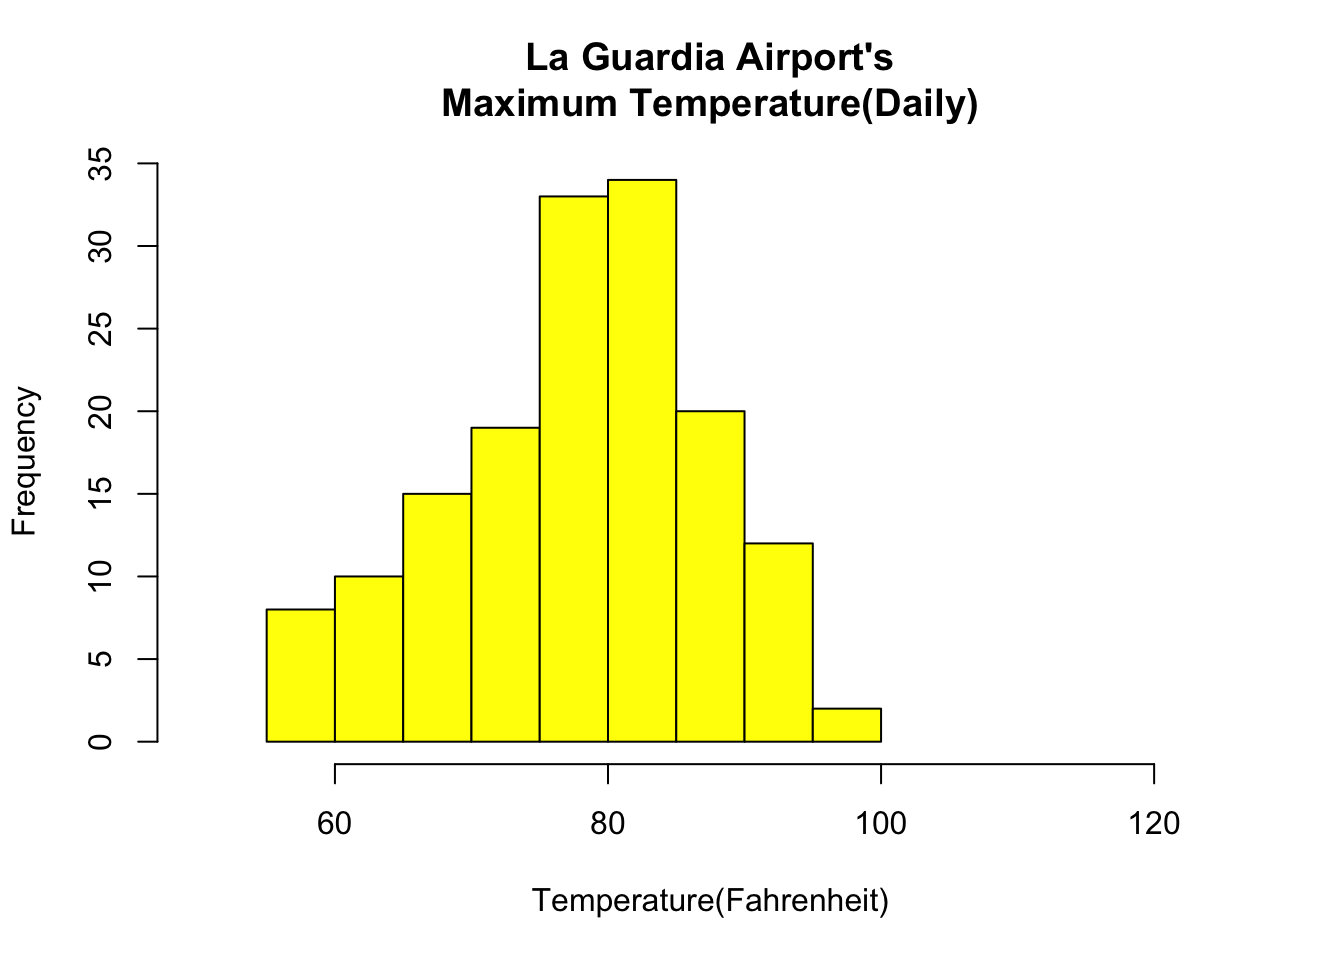
\includegraphics{./assignment1_files/figure-pdf/unnamed-chunk-1-1.pdf}

}

\end{figure}

\begin{Shaded}
\begin{Highlighting}[]
\DocumentationTok{\#\#\# Box Plot}

\FunctionTok{data}\NormalTok{(airquality)}
  
\FunctionTok{boxplot}\NormalTok{(airquality}\SpecialCharTok{$}\NormalTok{Wind, }\AttributeTok{main =} \StringTok{"Average wind speed\textbackslash{}}
\StringTok{at La Guardia Airport"}\NormalTok{,}
        \AttributeTok{xlab =} \StringTok{"Miles per hour"}\NormalTok{, }\AttributeTok{ylab =} \StringTok{"Wind"}\NormalTok{,}
        \AttributeTok{col =} \StringTok{"orange"}\NormalTok{, }\AttributeTok{border =} \StringTok{"brown"}\NormalTok{,}
        \AttributeTok{horizontal =} \ConstantTok{TRUE}\NormalTok{, }\AttributeTok{notch =} \ConstantTok{TRUE}\NormalTok{)}
\end{Highlighting}
\end{Shaded}

\begin{figure}[H]

{\centering 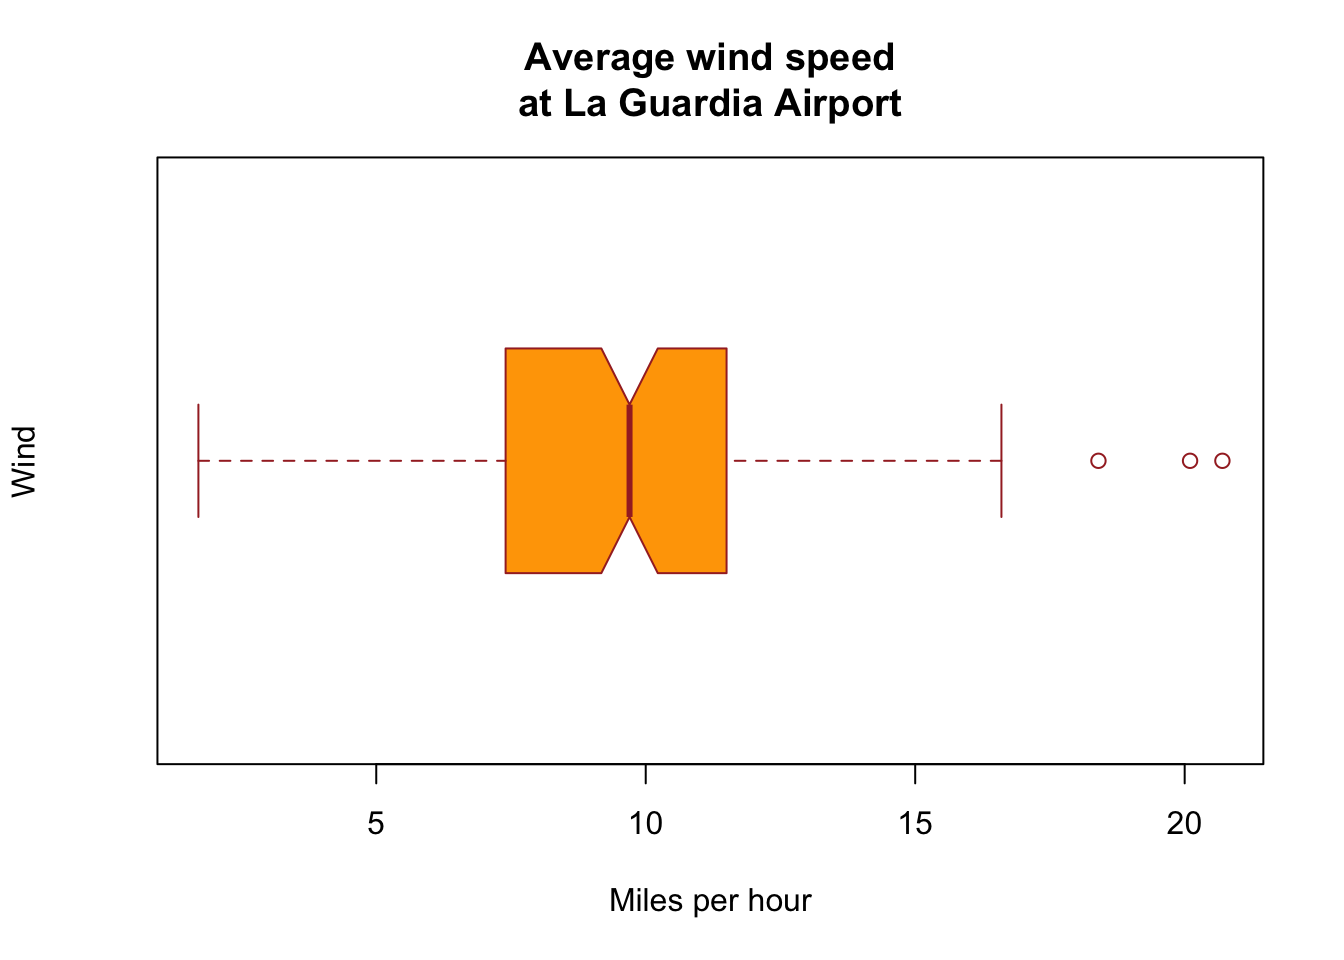
\includegraphics{./assignment1_files/figure-pdf/unnamed-chunk-1-2.pdf}

}

\end{figure}

\begin{Shaded}
\begin{Highlighting}[]
\DocumentationTok{\#\#\# Scatter Plot}

\FunctionTok{data}\NormalTok{(airquality)}
  
\FunctionTok{plot}\NormalTok{(airquality}\SpecialCharTok{$}\NormalTok{Ozone, airquality}\SpecialCharTok{$}\NormalTok{Month,}
     \AttributeTok{main =}\StringTok{"Scatterplot Example"}\NormalTok{,}
    \AttributeTok{xlab =}\StringTok{"Ozone Concentration in parts per billion"}\NormalTok{,}
    \AttributeTok{ylab =}\StringTok{" Month of observation "}\NormalTok{, }\AttributeTok{pch =} \DecValTok{19}\NormalTok{)}
\end{Highlighting}
\end{Shaded}

\begin{figure}[H]

{\centering 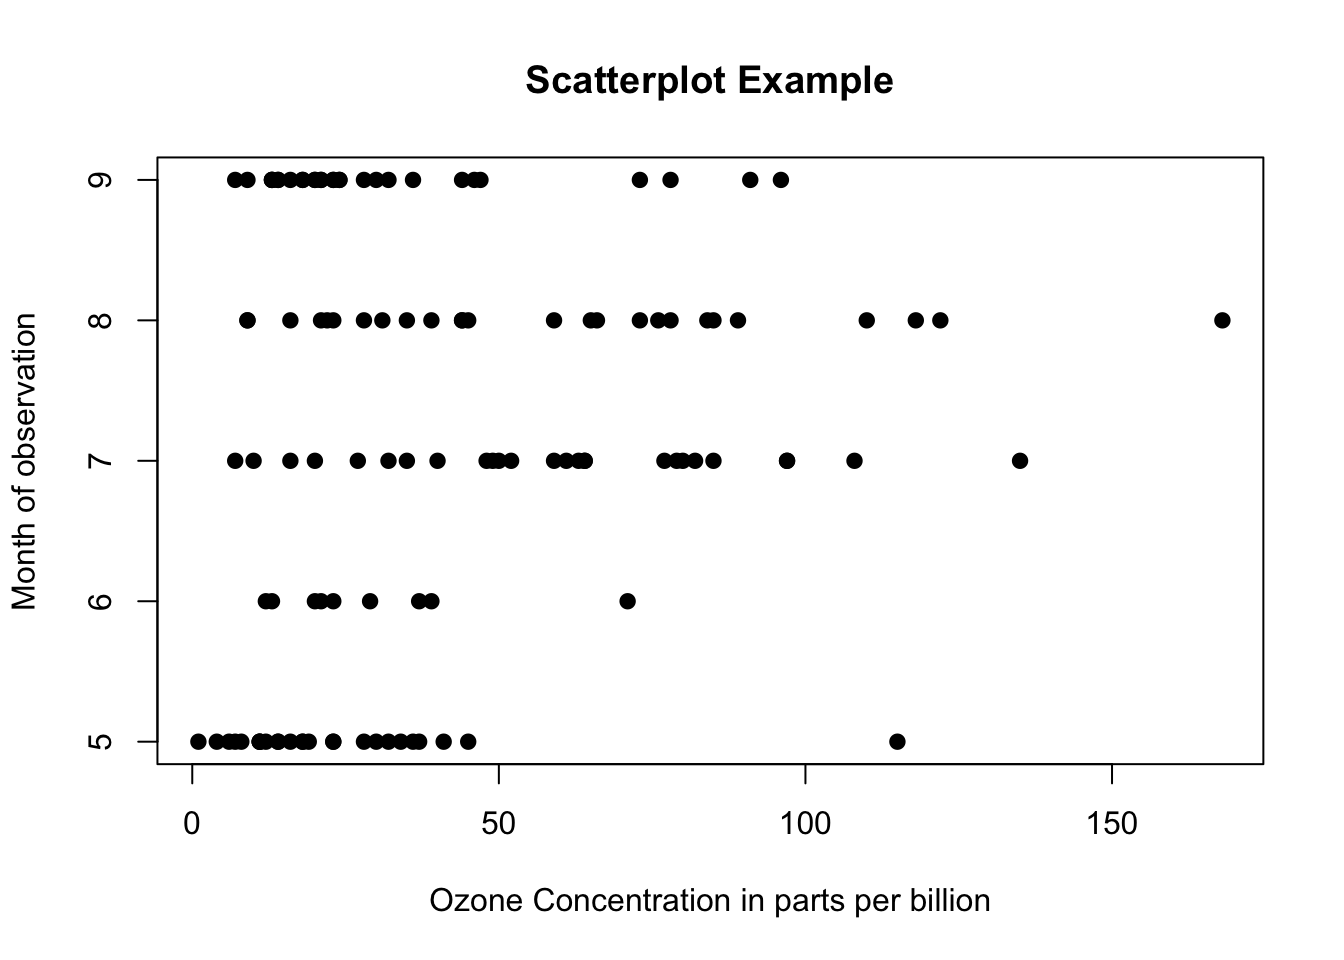
\includegraphics{./assignment1_files/figure-pdf/unnamed-chunk-1-3.pdf}

}

\end{figure}

\begin{Shaded}
\begin{Highlighting}[]
\DocumentationTok{\#\#\# Heat Map}

\CommentTok{\# Set seed for reproducibility}
\CommentTok{\# set.seed(110)}
  
\CommentTok{\# Create example data}
\NormalTok{data }\OtherTok{\textless{}{-}} \FunctionTok{matrix}\NormalTok{(}\FunctionTok{rnorm}\NormalTok{(}\DecValTok{50}\NormalTok{, }\DecValTok{0}\NormalTok{, }\DecValTok{5}\NormalTok{), }\AttributeTok{nrow =} \DecValTok{5}\NormalTok{, }\AttributeTok{ncol =} \DecValTok{5}\NormalTok{)}
\end{Highlighting}
\end{Shaded}

\begin{verbatim}
Warning in matrix(rnorm(50, 0, 5), nrow = 5, ncol = 5): data length differs from
size of matrix: [50 != 5 x 5]
\end{verbatim}

\begin{Shaded}
\begin{Highlighting}[]
\CommentTok{\# Column names}
\FunctionTok{colnames}\NormalTok{(data) }\OtherTok{\textless{}{-}} \FunctionTok{paste0}\NormalTok{(}\StringTok{"col"}\NormalTok{, }\DecValTok{1}\SpecialCharTok{:}\DecValTok{5}\NormalTok{)}
\FunctionTok{rownames}\NormalTok{(data) }\OtherTok{\textless{}{-}} \FunctionTok{paste0}\NormalTok{(}\StringTok{"row"}\NormalTok{, }\DecValTok{1}\SpecialCharTok{:}\DecValTok{5}\NormalTok{)}
  
\CommentTok{\# Draw a heatmap}
\FunctionTok{heatmap}\NormalTok{(data)     }
\end{Highlighting}
\end{Shaded}

\begin{figure}[H]

{\centering 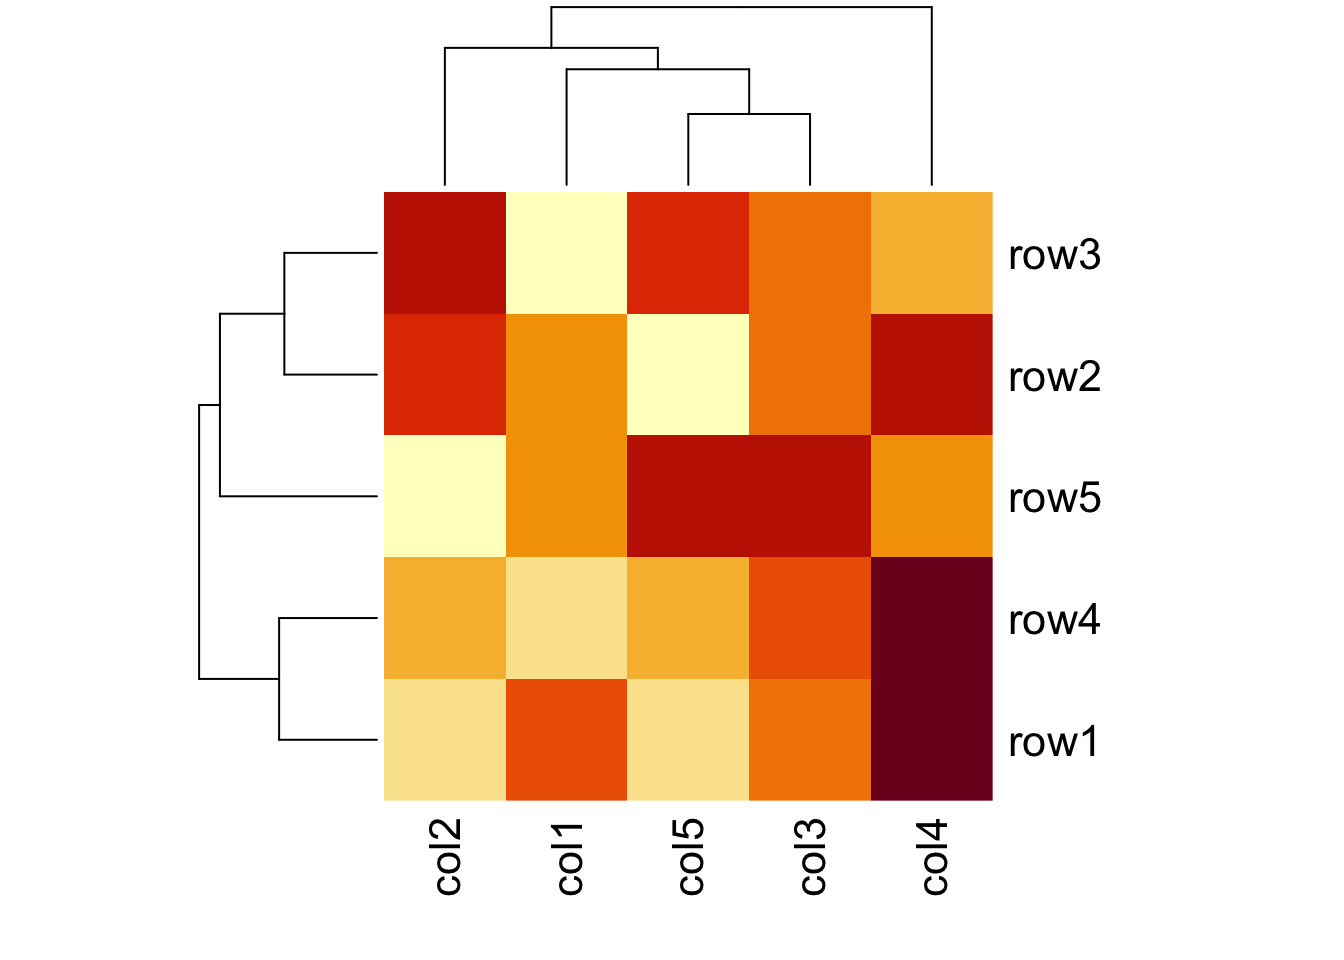
\includegraphics{./assignment1_files/figure-pdf/unnamed-chunk-1-4.pdf}

}

\end{figure}

\href{https://www.geeksforgeeks.org/data-visualization-in-r}{\emph{reference
for the basic visualization with R}}

\hypertarget{logistic-regression-in-r}{%
\subsection{Logistic Regression in R}\label{logistic-regression-in-r}}

Logistic regression is one of the most popular model for classification
problems. In this part i examined how can we use this algorithm in R.

For this example, we'll use the Default dataset from the ISLR package.
We can use the following code to load and view a summary of the dataset:

\begin{Shaded}
\begin{Highlighting}[]
\FunctionTok{options}\NormalTok{(}\AttributeTok{repos=}\StringTok{"https://cran.rstudio.com"}\NormalTok{ )}
\FunctionTok{install.packages}\NormalTok{(}\StringTok{"ISLR"}\NormalTok{)}
\end{Highlighting}
\end{Shaded}

\begin{verbatim}

The downloaded binary packages are in
    /var/folders/z6/nz1bbvyn06z34736vzgsqm_40000gn/T//Rtmpi64zr6/downloaded_packages
\end{verbatim}

\begin{Shaded}
\begin{Highlighting}[]
\FunctionTok{library}\NormalTok{(}\StringTok{"ISLR"}\NormalTok{)}

\NormalTok{data }\OtherTok{\textless{}{-}}\NormalTok{ ISLR}\SpecialCharTok{::}\NormalTok{Default}

\FunctionTok{summary}\NormalTok{(data)}
\end{Highlighting}
\end{Shaded}

\begin{verbatim}
 default    student       balance           income     
 No :9667   No :7056   Min.   :   0.0   Min.   :  772  
 Yes: 333   Yes:2944   1st Qu.: 481.7   1st Qu.:21340  
                       Median : 823.6   Median :34553  
                       Mean   : 835.4   Mean   :33517  
                       3rd Qu.:1166.3   3rd Qu.:43808  
                       Max.   :2654.3   Max.   :73554  
\end{verbatim}

Next, we'll split the dataset into a training set to train the model on
and a testing set to test the model on.

\begin{Shaded}
\begin{Highlighting}[]
\CommentTok{\#make this example reproducible}
\FunctionTok{set.seed}\NormalTok{(}\DecValTok{1}\NormalTok{)}

\CommentTok{\#Use 70\% of dataset as training set and remaining 30\% as testing set}
\NormalTok{sample }\OtherTok{\textless{}{-}} \FunctionTok{sample}\NormalTok{(}\FunctionTok{c}\NormalTok{(}\ConstantTok{TRUE}\NormalTok{, }\ConstantTok{FALSE}\NormalTok{), }\FunctionTok{nrow}\NormalTok{(data), }\AttributeTok{replace=}\ConstantTok{TRUE}\NormalTok{, }\AttributeTok{prob=}\FunctionTok{c}\NormalTok{(}\FloatTok{0.7}\NormalTok{,}\FloatTok{0.3}\NormalTok{))}
\NormalTok{train }\OtherTok{\textless{}{-}}\NormalTok{ data[sample, ]}
\NormalTok{test }\OtherTok{\textless{}{-}}\NormalTok{ data[}\SpecialCharTok{!}\NormalTok{sample, ]   }
\end{Highlighting}
\end{Shaded}

Next, we'll use the glm (general linear model) function and specify
family=``binomial'' so that R fits a logistic regression model to the
dataset:

\begin{Shaded}
\begin{Highlighting}[]
\CommentTok{\#fit logistic regression model}

\NormalTok{model }\OtherTok{\textless{}{-}} \FunctionTok{glm}\NormalTok{(default}\SpecialCharTok{\textasciitilde{}}\NormalTok{student}\SpecialCharTok{+}\NormalTok{balance}\SpecialCharTok{+}\NormalTok{income, }\AttributeTok{family=}\StringTok{"binomial"}\NormalTok{, }\AttributeTok{data=}\NormalTok{train)}

\CommentTok{\#disable scientific notation for model summary}
\FunctionTok{options}\NormalTok{(}\AttributeTok{scipen=}\DecValTok{999}\NormalTok{)}

\CommentTok{\#view model summary}
\FunctionTok{summary}\NormalTok{(model)}
\end{Highlighting}
\end{Shaded}

\begin{verbatim}

Call:
glm(formula = default ~ student + balance + income, family = "binomial", 
    data = train)

Deviance Residuals: 
    Min       1Q   Median       3Q      Max  
-2.5586  -0.1353  -0.0519  -0.0177   3.7973  

Coefficients:
                 Estimate    Std. Error z value            Pr(>|z|)    
(Intercept) -11.478101194   0.623409555 -18.412 <0.0000000000000002 ***
studentYes   -0.493292438   0.285735949  -1.726              0.0843 .  
balance       0.005988059   0.000293765  20.384 <0.0000000000000002 ***
income        0.000007857   0.000009965   0.788              0.4304    
---
Signif. codes:  0 '***' 0.001 '**' 0.01 '*' 0.05 '.' 0.1 ' ' 1

(Dispersion parameter for binomial family taken to be 1)

    Null deviance: 2021.1  on 6963  degrees of freedom
Residual deviance: 1065.4  on 6960  degrees of freedom
AIC: 1073.4

Number of Fisher Scoring iterations: 8
\end{verbatim}

\begin{Shaded}
\begin{Highlighting}[]
\FunctionTok{glm}\NormalTok{(}\AttributeTok{formula =}\NormalTok{ default }\SpecialCharTok{\textasciitilde{}}\NormalTok{ student }\SpecialCharTok{+}\NormalTok{ balance }\SpecialCharTok{+}\NormalTok{ income, }\AttributeTok{family =} \StringTok{"binomial"}\NormalTok{, }
    \AttributeTok{data =}\NormalTok{ train)}
\end{Highlighting}
\end{Shaded}

\begin{verbatim}

Call:  glm(formula = default ~ student + balance + income, family = "binomial", 
    data = train)

Coefficients:
  (Intercept)     studentYes        balance         income  
-11.478101194   -0.493292438    0.005988059    0.000007857  

Degrees of Freedom: 6963 Total (i.e. Null);  6960 Residual
Null Deviance:      2021 
Residual Deviance: 1065     AIC: 1073
\end{verbatim}

The coefficients in the output indicate the average change in log odds
of defaulting. For example, a one unit increase in balance is associated
with an average increase of 0.005988 in the log odds of defaulting.

The p-values in the output also give us an idea of how effective each
predictor variable is at predicting the probability of default:

P-value of student status: 0.0843

P-value of balance: \textless0.0000

P-value of income: 0.4304

Use the Model to Make Predictions:

\begin{Shaded}
\begin{Highlighting}[]
\CommentTok{\#define two individuals}
\NormalTok{new }\OtherTok{\textless{}{-}} \FunctionTok{data.frame}\NormalTok{(}\AttributeTok{balance =} \DecValTok{1400}\NormalTok{, }\AttributeTok{income =} \DecValTok{2000}\NormalTok{, }\AttributeTok{student =} \FunctionTok{c}\NormalTok{(}\StringTok{"Yes"}\NormalTok{, }\StringTok{"No"}\NormalTok{))}

\CommentTok{\#predict probability of defaulting}
\FunctionTok{predict}\NormalTok{(model, new, }\AttributeTok{type=}\StringTok{"response"}\NormalTok{)}
\end{Highlighting}
\end{Shaded}

\begin{verbatim}
         1          2 
0.02732106 0.04397747 
\end{verbatim}

\href{https://www.statology.org/logistic-regression-in-r/}{\emph{reference
for the logistic regression with R}}

\hypertarget{lag-lead-r-functions}{%
\subsection{LAG \& LEAD R Functions}\label{lag-lead-r-functions}}

Firstly we have to install and load dplyr package:

\begin{Shaded}
\begin{Highlighting}[]
\FunctionTok{install.packages}\NormalTok{(}\StringTok{"dplyr"}\NormalTok{)       }
\end{Highlighting}
\end{Shaded}

\begin{verbatim}

The downloaded binary packages are in
    /var/folders/z6/nz1bbvyn06z34736vzgsqm_40000gn/T//Rtmpi64zr6/downloaded_packages
\end{verbatim}

\begin{Shaded}
\begin{Highlighting}[]
\FunctionTok{library}\NormalTok{(}\StringTok{"dplyr"}\NormalTok{)     }
\end{Highlighting}
\end{Shaded}

\begin{verbatim}

Attaching package: 'dplyr'
\end{verbatim}

\begin{verbatim}
The following objects are masked from 'package:stats':

    filter, lag
\end{verbatim}

\begin{verbatim}
The following objects are masked from 'package:base':

    intersect, setdiff, setequal, union
\end{verbatim}

And giving an example vector as x :

\begin{Shaded}
\begin{Highlighting}[]
\NormalTok{x}\OtherTok{\textless{}{-}} \DecValTok{1}\SpecialCharTok{:}\DecValTok{10}
\end{Highlighting}
\end{Shaded}

Here is the basic application for lag and lead

\begin{Shaded}
\begin{Highlighting}[]
\DocumentationTok{\#\#Lead :}

\FunctionTok{lead}\NormalTok{(x)}
\end{Highlighting}
\end{Shaded}

\begin{verbatim}
 [1]  2  3  4  5  6  7  8  9 10 NA
\end{verbatim}

\begin{Shaded}
\begin{Highlighting}[]
\DocumentationTok{\#\#Lag :}

\FunctionTok{lag}\NormalTok{(x)}
\end{Highlighting}
\end{Shaded}

\begin{verbatim}
 [1] NA  1  2  3  4  5  6  7  8  9
\end{verbatim}

\href{https://statisticsglobe.com/r-lead-lag-functions-dplyr-package}{\emph{reference
for the lag and lead functions}}

\bookmarksetup{startatroot}

\hypertarget{inclass-exercise-1}{%
\chapter{Inclass Exercise-1}\label{inclass-exercise-1}}

After installation step we have to call the packages :

\begin{Shaded}
\begin{Highlighting}[]
\FunctionTok{library}\NormalTok{(tidyverse)}
\FunctionTok{library}\NormalTok{(nycflights13)}
\end{Highlighting}
\end{Shaded}

First, we take a look at the data to see how many columns and rows we
have, as well as what types of data we have :

\begin{Shaded}
\begin{Highlighting}[]
\FunctionTok{glimpse}\NormalTok{(planes)}
\end{Highlighting}
\end{Shaded}

\begin{verbatim}
Rows: 3,322
Columns: 9
$ tailnum      <chr> "N10156", "N102UW", "N103US", "N104UW", "N10575", "N105UW~
$ year         <int> 2004, 1998, 1999, 1999, 2002, 1999, 1999, 1999, 1999, 199~
$ type         <chr> "Fixed wing multi engine", "Fixed wing multi engine", "Fi~
$ manufacturer <chr> "EMBRAER", "AIRBUS INDUSTRIE", "AIRBUS INDUSTRIE", "AIRBU~
$ model        <chr> "EMB-145XR", "A320-214", "A320-214", "A320-214", "EMB-145~
$ engines      <int> 2, 2, 2, 2, 2, 2, 2, 2, 2, 2, 2, 2, 2, 2, 2, 2, 2, 2, 2, ~
$ seats        <int> 55, 182, 182, 182, 55, 182, 182, 182, 182, 182, 55, 55, 5~
$ speed        <int> NA, NA, NA, NA, NA, NA, NA, NA, NA, NA, NA, NA, NA, NA, N~
$ engine       <chr> "Turbo-fan", "Turbo-fan", "Turbo-fan", "Turbo-fan", "Turb~
\end{verbatim}

In ``plane'' dataset we have information about each plane's
construction.

\begin{Shaded}
\begin{Highlighting}[]
\NormalTok{planes }\SpecialCharTok{\%\textgreater{}\%} 
  \FunctionTok{filter}\NormalTok{(manufacturer }\SpecialCharTok{==} \StringTok{"AIRBUS INDUSTRIE"}\NormalTok{) }\SpecialCharTok{\%\textgreater{}\%} 
  \FunctionTok{group\_by}\NormalTok{(seats) }\SpecialCharTok{\%\textgreater{}\%} 
  \FunctionTok{summarise}\NormalTok{(}\AttributeTok{count\_of\_planes =} \FunctionTok{n}\NormalTok{()) }\SpecialCharTok{\%\textgreater{}\%} 
  \FunctionTok{arrange}\NormalTok{(}\FunctionTok{desc}\NormalTok{(count\_of\_planes))}
\end{Highlighting}
\end{Shaded}

\begin{verbatim}
# A tibble: 7 x 2
  seats count_of_planes
  <int>           <int>
1   200             127
2   179             124
3   182              94
4   145              26
5   199              25
6   379               3
7   375               1
\end{verbatim}

\hypertarget{for-each-manufacturer-oldest-newest-plane-model-and-counts}{%
\subsection{For each manufacturer oldest, newest plane model and
counts}\label{for-each-manufacturer-oldest-newest-plane-model-and-counts}}

\begin{Shaded}
\begin{Highlighting}[]
\NormalTok{planes }\SpecialCharTok{\%\textgreater{}\%} 
  \FunctionTok{group\_by}\NormalTok{(manufacturer) }\SpecialCharTok{\%\textgreater{}\%} 
  \FunctionTok{summarise}\NormalTok{(}\AttributeTok{min\_model\_year =} \FunctionTok{min}\NormalTok{(year, }\AttributeTok{na.rm =}\NormalTok{ T), }\AttributeTok{max\_model\_year =} \FunctionTok{max}\NormalTok{(year, }\AttributeTok{na.rm =}\NormalTok{ T),}\AttributeTok{distinct\_plane\_counts =}\FunctionTok{n\_distinct}\NormalTok{(tailnum)) }\SpecialCharTok{\%\textgreater{}\%} 
  \FunctionTok{arrange}\NormalTok{(manufacturer)  }\SpecialCharTok{\%\textgreater{}\%}
  \FunctionTok{print}\NormalTok{(}\AttributeTok{n =} \ConstantTok{Inf}\NormalTok{) }
\end{Highlighting}
\end{Shaded}

\begin{verbatim}
# A tibble: 35 x 4
   manufacturer                  min_model_year max_model_year distinct_plane_~1
   <chr>                                  <dbl>          <dbl>             <int>
 1 AGUSTA SPA                              2001           2001                 1
 2 AIRBUS                                  2002           2013               336
 3 AIRBUS INDUSTRIE                        1989           2013               400
 4 AMERICAN AIRCRAFT INC                    Inf           -Inf                 2
 5 AVIAT AIRCRAFT INC                      2007           2007                 1
 6 AVIONS MARCEL DASSAULT                  1986           1986                 1
 7 BARKER JACK L                            Inf           -Inf                 1
 8 BEECH                                   1967           1972                 2
 9 BELL                                    1975           1994                 2
10 BOEING                                  1965           2013              1630
11 BOMBARDIER INC                          1998           2013               368
12 CANADAIR                                1997           1998                 9
13 CANADAIR LTD                            1974           1974                 1
14 CESSNA                                  1959           1983                 9
15 CIRRUS DESIGN CORP                      2007           2007                 1
16 DEHAVILLAND                             1959           1959                 1
17 DOUGLAS                                 1956           1956                 1
18 EMBRAER                                 1998           2013               299
19 FRIEDEMANN JON                          2007           2007                 1
20 GULFSTREAM AEROSPACE                    1976           1992                 2
21 HURLEY JAMES LARRY                       Inf           -Inf                 1
22 JOHN G HESS                              Inf           -Inf                 1
23 KILDALL GARY                            1985           1985                 1
24 LAMBERT RICHARD                          Inf           -Inf                 1
25 LEARJET INC                              Inf           -Inf                 1
26 LEBLANC GLENN T                         1985           1985                 1
27 MARZ BARRY                              1993           1993                 1
28 MCDONNELL DOUGLAS                       1975           1998               120
29 MCDONNELL DOUGLAS AIRCRAFT CO           1987           1993               103
30 MCDONNELL DOUGLAS CORPORATION           1991           1992                14
31 PAIR MIKE E                              Inf           -Inf                 1
32 PIPER                                   1968           1980                 5
33 ROBINSON HELICOPTER CO                  2012           2012                 1
34 SIKORSKY                                1985           1985                 1
35 STEWART MACO                            1985           1985                 2
# ... with abbreviated variable name 1: distinct_plane_counts
\end{verbatim}

\begin{center}\rule{0.5\linewidth}{0.5pt}\end{center}

\bookmarksetup{startatroot}

\hypertarget{shiny_foreign_students}{%
\chapter{Shiny\_Foreign\_Students}\label{shiny_foreign_students}}

We've been given a dataset about foreign students who are in Turkey.
After some data cleaning and analysis processes I've prepared a Shiny
app.

It consists of two separates tabs: ``The distribution of top N foreign
students by their nations'' and ``Foreign Student's Distribution by
Province''

\hypertarget{shinyapps.io}{%
\subsection{shinyapps.io}\label{shinyapps.io}}

\url{https://mef06-berkozzcan.shinyapps.io/shiny_assignment/}

\hypertarget{command-for-local-running}{%
\subsection{Command for local running}\label{command-for-local-running}}

\begin{Shaded}
\begin{Highlighting}[]
\NormalTok{shiny}\SpecialCharTok{::}\FunctionTok{runGitHub}\NormalTok{(}\AttributeTok{repo =} \StringTok{"pjournal/mef06{-}berkozzcan"}\NormalTok{,}\AttributeTok{subdir=}\StringTok{"/Shiny\_Assignment"}\NormalTok{)}
\end{Highlighting}
\end{Shaded}

\bookmarksetup{startatroot}

\hypertarget{or-case-study}{%
\chapter{OR Case Study}\label{or-case-study}}

\href{https://www.gurobi.com/case_studies/toyota-production-planning-optimization/}{Here
is the chosen case study.}

\hypertarget{business-case}{%
\section{Business Case}\label{business-case}}

An automaker brand Toyota aims to produce highly profitable models and
ensure that these models comply with environmental regulations. To
achieve this, Toyota spent an immense amount of time and effort, the
managers used excel and they ran manually multiple simulations.

\hypertarget{problem}{%
\section{Problem}\label{problem}}

Toyota needs to determine automatically and in a short amount of time
the right product mix to maximize the profitability while the brand is
ensuring environmental compliance.

\hypertarget{solution}{%
\section{Solution}\label{solution}}

For solving this problem Toyota decided to use mathematical optimization
to find out optimal product mix. The brand evaluated several
mathematical optimization solvers and after that they chose Gurobi
Optimizer. ( Gurobi calls themselves ``the fastest solver on the market
today'' ) The Gurobi Optimizer is used to perform simulations thus the
environmental regulations in each country and region are taken into
account. After simulations are made the result feed into Toyota's Profit
Planning Module and finally they can run additional simulations to
calculate projected profit for the next fiscal year.



\end{document}
